\documentclass[a4paper,11pt, twoside]{memoir}

\usepackage{unicode-math}
\usepackage{amsmath}
\usepackage{lualatex-math}
\usepackage{polyglossia}
\setdefaultlanguage{polish}
\defaultfontfeatures{Ligatures=TeX}

\usepackage[top=25mm, bottom=25mm, left=30mm, right=20mm]{geometry}
\usepackage[linktoc=section]{hyperref}
\hypersetup{verbose, pdfborder={0 0 0.2},   bookmarksopen=true ,bookmarksnumbered=true, colorlinks=false,  unicode=true}
\usepackage{bookmark}
\usepackage[usenames,dvipsnames]{color}
\usepackage{url}
\usepackage{listings}
\usepackage[sort, compress]{cite}
\usepackage{graphicx}
\usepackage[labelsep=period]{caption}
\usepackage{diagbox}
\usepackage{xfrac}
\usepackage{tabularx}
\usepackage{setspace}
\usepackage{fontspec}
\usepackage{siunitx, booktabs}
\usepackage{nicefrac}
\defaultfontfeatures{Ligatures=TeX}






%%%%%%%%%%%%%%%%%%%%%%%%%%%%%%%%%%%%%%%%%%%%%%%%%%%%%%%%%%%%%%%%%%%%%%%%%%%%%%%%%%%%%%%%%
%%% Wybór fontu)                                                                      %%%
%%%\setmainfont{TeX Gyre Pagella})                                                    %%%
\setmainfont{FreeSerif}                                                               %%%
%%%%%%%%%%%%%%%%%%%%%%%%%%%%%%%%%%%%%%%%%%%%%%%%%%%%%%%%%%%%%%%%%%%%%%%%%%%%%%%%%%%%%%%%%


%%%%%%%%%%%%%%%%%%%%%%%%%%%%%%%%%%%%%%%%%%%%%%%%%%%%%%%%%%%%%%%%%%%%%%%%%%%%%%%%%%%%%%%%%
%%% Definicje symboli i skrótów (początek)                                            %%%
\usepackage[toc, nonumberlist]{glossaries}                                            %%%
\usepackage{glossaries-extra}                                                         %%%
\setglossarystyle{listdotted}                                                         %%%
\setlength{\glslistdottedwidth}{25mm}                                                 %%%

\makenoidxglossaries                                                                  %%%
\loadglsentries{glossary.tex}                                                         %%%
\glsaddall                                                                            %%%
%%% Definicje symboli i skrótów (koniec)                                              %%%
%%%%%%%%%%%%%%%%%%%%%%%%%%%%%%%%%%%%%%%%%%%%%%%%%%%%%%%%%%%%%%%%%%%%%%%%%%%%%%%%%%%%%%%%%


%%%%%%%%%%%%%%%%%%%%%%%%%%%%%%%%%%%%%%%%%%%%%%%%%%%%%%%%%%%%%%%%%%%%%%%%%%%%%%%%%%%%%%%%%
%%% Pomocnicze makro definiujące elegancką werję  BibTeX                              %%%
\def\BibTeX{{\textrm B\kern-.05em{\textsc i\kern-.025em b}\kern-.08emT\kern-.1667em\lower.5ex\hbox{E}\kern-.125emX }}                         %%%
%%%%%%%%%%%%%%%%%%%%%%%%%%%%%%%%%%%%%%%%%%%%%%%%%%%%%%%%%%%%%%%%%%%%%%%%%%%%%%%%%%%%%%%%%


%%%%%%%%%%%%%%%%%%%%%%%%%%%%%%%%%%%%%%%%%%%%%%%%%%%%%%%%%%%%%%%%%%%%%%%%%%%%%%%%%%%%%%%%%
%%%   Tabele i rysunki                                                                %%%
%%%Parametr "rozciągający" komórki tabeli                                             %%%
%\renewcommand{\arraystretch}{1.2}                                                    %%%
                                                                                      %%%
%%% dodatkowy odstęp w tablicy                                                        %%%
\setlength\extrarowheight{2pt}                                                        %%%
                                                                                      %%%
%%% Format podpisów rysunków                                                          %%%
\captionsetup[figure]{skip=0pt, name=Rys.}                                            %%%
%%%%%%%%%%%%%%%%%%%%%%%%%%%%%%%%%%%%%%%%%%%%%%%%%%%%%%%%%%%%%%%%%%%%%%%%%%%%%%%%%%%%%%%%%


%%%%%%%%%%%%%%%%%%%%%%%%%%%%%%%%%%%%%%%%%%%%%%%%%%%%%%%%%%%%%%%%%%%%%%%%%%%%%%%%%%%%%%%%%
%%% Konfiguracja głębokości numeracji podrozdziałów
\setsecnumdepth{subsection}
\maxsecnumdepth{subsection}

%%% Konfiguracja głębokości spisu treści
%%% Dwa poziomy
\maxtocdepth{section}
%%% lub
%%% trzy poziomy 
%\maxtocdepth{subsection}

%%%Lokalizacja plików graficznych
%%%%%%%%%%%%%%%%%%%%%%%%%%%%%%%%%%%%%%%%%%%%%%%%%%%%%%%%%%%%%%%%%%%%%%%%%%%%%%%%%%%%%%%%%
\graphicspath{ {./grafika/} }
%%%%%%%%%%%%%%%%%%%%%%%%%%%%%%%%%%%%%%%%%%%%%%%%%%%%%%%%%%%%%%%%%%%%%%%%%%%%%%%%%%%%%%%%%


%%%%%%%%%%%%%%%%%%%%%%%%%%%%%%%%%%%%%%%%%%%%%%%%%%%%%%%%%%%%%%%%%%%%%%%%%%%%%%%%%%%%%%%%%

%%%%%%%%%%%%%%%%%%%%%%%%%%%%%%%%%%%%%%%%%%%%%%%%%%%%%%%%%%%%%%%%%%%%%%%%%%%%%%%%%%%%%%%%%

%%%%%%%%%%%%%%%%%%%%%%%%%%%%%%%%%%%%%%%%%%%%%%%%%%%%%%%%%%%%%%%%%%%%%%%%%%%%%%%%%%%%%%%%%
%%%  Parametry wpływające na skład tekstu                                             %%%
\clubpenalty=10000                                                                    %%%
\widowpenalty=10000                                                                   %%%
\brokenpenalty=10000                                                                  %%%
\sloppy                                                                               %%%
                                                                                      %%%
\tolerance4500                                                                        %%%
\pretolerance250                                                                      %%%
\hfuzz=1.5pt                                                                          %%%
\hbadness1450                                                                         %%%
%%%%%%%%%%%%%%%%%%%%%%%%%%%%%%%%%%%%%%%%%%%%%%%%%%%%%%%%%%%%%%%%%%%%%%%%%%%%%%%%%%%%%%%%%


%%%%%%%%%%%%%%%%%%%%%%%%%%%%%%%%%%%%%%%%%%%%%%%%%%%%%%%%%%%%%%%%%%%%%%%%%%%%%%%%%%%%%%%%%
%%% Definiowanie stylu strony (początek)                                              %%%
\chapterstyle{section}                                                                %%%
\copypagestyle{chapter}{ruled}                                                        %%%
\pagestyle{empty}                                                                     %%%
\makeevenhead{ruled}{}{}{}                                                            %%%
\makeoddhead{ruled}{}{}{}                                                             %%%
\makeheadrule{ruled}{0pt}{0pt}                                                        %%%
\setlength{\parindent}{5mm}                                                           %%%
%%%%%%%%%%%%%%%%%%%%%%%%%%%%%%%%%%%%%%%%%%%%%%%%%%%%%%%%%%%%%%%%%%%%%%%%%%%%%%%%%%%%%%%%%


%%%%%%%%%%%%%%%%%%%%%%%%%%%%%%%%%%%%%%%%%%%%%%%%%%%%%%%%%%%%%%%%%%%%%%%%%%%%%%%%%%%%%%%%%
%%% Symbole używane w listach                                                         %%%
\renewcommand{\labelitemi}{$\bullet$}                                                 %%%
\renewcommand{\labelitemii}{--}                                                       %%%
\renewcommand{\labelitemiii}{$\circ$}                                                 %%%
%%%%%%%%%%%%%%%%%%%%%%%%%%%%%%%%%%%%%%%%%%%%%%%%%%%%%%%%%%%%%%%%%%%%%%%%%%%%%%%%%%%%%%%%%


%%%%%%%%%%%%%%%%%%%%%%%%%%%%%%%%%%%%%%%%%%%%%%%%%%%%%%%%%%%%%%%%%%%%%%%%%%%%%%%%%%%%%%%%%
\definecolor{ListingBackground}{rgb}{0.95,0.95,0.95}                                  %%%
\lstset{ %language=VHDL,                                                              %%%
	basicstyle=\scriptsize,                                                           %%%
	frameround=ffff,                                                                  %%%
	keywordstyle={\bfseries\scriptsize},                                              %%%
	commentstyle={\em\scriptsize\color{Gray}},                                        %%%
	numbers=left,                                                                     %%%
	stepnumber=5,                                                                     %%%
	firstnumber=1,                                                                    %%%
	numberfirstline=true,                                                             %%%
	numberblanklines=true,                                                            %%%
	numberstyle={\tiny},                                                              %%%
	numbersep=10pt,                                                                   %%%
	tabsize=2,                                                                        %%%
	xleftmargin=20pt,                                                                 %%%
	framexleftmargin=3pt,                                                             %%%
	framexbottommargin=2pt,                                                           %%%
	framextopmargin=2pt,                                                              %%%
	framexrightmargin=0pt,                                                            %%%
	showstringspaces=true,                                                            %%%
	backgroundcolor={\color{ListingBackground}},                                      %%%
	extendedchars=true,                                                               %%%
	% title=\lstname,                                                                 %%%
	captionpos=t,                                                                     %%%
	% abovecaptionskip=1pt,                                                           %%%
	% belowcaptionskip=1pt,                                                           %%%
	frame=tb,                                                                         %%%
	framerule=0.2pt}                                                                  %%%
%%%%%%%%%%%%%%%%%%%%%%%%%%%%%%%%%%%%%%%%%%%%%%%%%%%%%%%%%%%%%%%%%%%%%%%%%%%%%%%%%%%%%%%%%


%%%%%%%%%%%%%%%%%%%%%%%%%%%%%%%%%%%%%%%%%%%%%%%%%%%%%%%%%%%%%%%%%%%%%%%%%%%%%%%%%%%%%%%%%
%%% Spolszczone/zmienione nazwy sekcji dokumentu                                      %%%
\renewcommand*\lstlistingname{Wydruk}                                                 %%%
\renewcommand*\lstlistlistingname{Spis wydruków}                                      %%%
                                                                                      %%%
\renewcommand{\appendixname}{Załącznik}                                               %%%
\renewcommand{\appendixpagename}{Załączniki}                                          %%%
%\renewcommand{\appendixpagename}{załączniki}                                          %%%

\renewcommand{\appendixtocname}{Spis załączników}
%%%%%%%%%%%%%%%%%%%%%%%%%%%%%%%%%%%%%%%%%%%%%%%%%%%%%%%%%%%%%%%%%%%%%%%%%%%%%%%%%%%%%%%%%


\renewcommand\mempostaddapppagetotochook{\cftinserthook{toc}{BREAK}}
\cftinsertcode{BREAK}{\changetocdepth{-10}}
\let\normalchangetocdepth\changetocdepth
% needed for late

\makeatletter
\newcommand\appendixtableofcontents{
\begingroup
\let\changetocdepth\@gobble
\normalchangetocdepth{-10}
\cftinsertcode{BREAK}{\normalchangetocdepth{3}}
\renewcommand\contentsname{Spis załączników}
\tableofcontents*
\endgroup
}
\makeatother

%\newcommand{\listanswername}{Spis załączników}
%\newlistof{listofanswers}{zalaczniki}{\listanswername}
%
%\newcounter{answer}[chapter]
%\renewcommand{\theanswer}{\arabic{answer}}
%\newcommand{\answer}[1]{
%\refstepcounter{answer}
%\par\noindent\textbf{Answer \theanswer. #1}
%\addcontentsline{ans}{answer}{\protect\numberline{\theanswer}#1}\par}



\begin{document}
%%%%%%%%%%%%%%%%%%%%%%%%%%%%%%%%%%%%%%%%%%%%%%%%%%%%%%%%%%%%%%%%%%%%%%%%%%%%%%%%%%%%%%%%%
%%%%%%%%%%%%%%%% Parametry strony tytułowej  %%%%%%%%%%%%%%%%%%%%%%%%%%%%%%%%%%%%%%%%%%%%
%%%%%%%%%%%%%%%%%%%%%%%%%%%%%%%%%%%%%%%%%%%%%%%%%%%%%%%%%%%%%%%%%%%%%%%%%%%%%%%%%%%%%%%%%
\newcommand\rok{2024}
\newcommand\rodzajpracy{Praca dyplomowa \\ \vskip6pt inżynierska}
%\newcommand\rodzajpracy{Praca dyplomowa \\ \vskip6pt magisterska}
\newcommand\kierunek{Elektronika i Telekomunikacja}
\newcommand\specjalnosc{Inżynieria Komputerowa}
\newcommand\tytulpl{Dedykowany system komunikacji z wykorzystaniem protokołu Lora}
\newcommand\tytulen{Dedicated communication system using Lora protocol}
\newcommand\autor{Emil Michalik}
\newcommand\nralbumu{280293}
\newcommand\promotor{dr inż. Marek Niewiński}
%%%%%%%%%%%%%%%%%%%%%%%%%%%%%%%%%%%%%%%%%%%%%%%%%%%%%%%%%%%%%%%%%%%%%%%%%%%%%%%%%%%%%%%%%


%%%%%%%%%%%%%%%%%%%%%%%%%%%%%%%%%%%%%%%%%%%%%%%%%%%%%%%%%%%%%%%%%%%%%%%%%%%%%%%%%%%%%%%%%
%%%%%%%%%%%%%%%%%%%%%%%%%%%%%%%%%%%%%%%%%%%%%%%%%%%%%%%%%%%%%%%%%%%%%%%%%%%%%%%%%%%%%%%%%
%%% wczytanie pliku z formatem strony tytułowej
\thispagestyle{empty}

{ \centering

{ %\setmainfont{t1xtt} 
%\setmainfont[]{Belgrano Regular} %\ttfamily 
\setmainfont{Latin Modern Mono}
%\setmainfont{Noto Serif}
\begin{minipage}[c]{\textwidth}
\centering
\begin{minipage}[c]{0.65\textwidth}   \centering
{\fontsize{23pt}{36pt}\selectfont {Politechnika Warszawska}} \vskip 4pt 
{\setmainfont[LetterSpace=35]{Latin Modern Mono} \fontsize{12pt}{24pt}   \selectfont  
 {WYDZIAŁ \hskip12pt ELEKTRONIKI \\  I \hskip12pt TECHNIK \hskip12pt INFORMACYJNYCH}}
\end{minipage}
\begin{minipage}[c]{0.18\textwidth}
\centering

\includegraphics[height=25mm]{pwlogo.png}
\end{minipage}
\end{minipage}
}

\vfill

{\setmainfont{Noto Sans} 
\begin{minipage}[c]{\textwidth}   \centering
{\fontsize{12pt}{24pt}\selectfont Instytut Mikroelektroniki i Optoelektroniki}
\end{minipage}}

\vfill

{ %\setmainfont{t1xtt} 
%\setmainfont[]{Belgrano Regular}
\setmainfont{Latin Modern Mono}
\begin{minipage}[c][][c]{\textwidth}   \centering
{\fontsize{37pt}{120pt} \selectfont \rodzajpracy} 
\end{minipage}}

\vfill

{\setmainfont{Noto Sans}
\begin{minipage}[c]{\textwidth}   \centering
{\fontsize{12pt}{24pt}\selectfont na kierunku \kierunek}\\  \vskip 6pt 
{\fontsize{12pt}{24pt}\selectfont w specjalności \specjalnosc}
\end{minipage}}

\vfill

{\setmainfont{Noto Sans} 
\begin{minipage}[c]{\textwidth}   \centering
{\fontsize{14pt}{36pt}\selectfont \tytulpl}
\end{minipage}}

\vfill

	 
{\setmainfont{Noto Sans} 
\begin{minipage}[c]{\textwidth}   \centering
{\fontsize{20pt}{28pt}\selectfont \autor}\\ \vskip 6pt
{\fontsize{12pt}{24pt}\selectfont Numer albumu \nralbumu}
\end{minipage}}

\vfill

{\setmainfont{Noto Sans} 
\begin{minipage}[c]{\textwidth}   \centering 
{\fontsize{12pt}{24pt}\selectfont promotor\\ \vskip 6pt \promotor}
\end{minipage}}

\vfill

{\setmainfont{Noto Sans} 
\begin{minipage}[b][][b]{\textwidth}   \centering
{\fontsize{12pt}{24pt}\selectfont WARSZAWA \rok}
\end{minipage}}
}



%%%%%%%%%%%%%%%%%%%%%%%%%%%%%%%%%%%%%%%%%%%%%%%%%%%%%%%%%%%%%%%%%%%%%%%%%%%%%%%%%%%%%%%%%
%%%wczytanie pliku zawierającego dedykację
% !TeX encoding = UTF-8
% !TeX spellcheck = pl_PL
\newpage
    \begin{center}
	{\large\bfseries Podziękowania}\par\bigskip\end{center}
Jestem bardzo wdzięczny	mojemu promotorowi za bezcenne rady.
Mojej babci Apolonii za wiarę we mnie.
Natomiast moim rodzicom za niekończące się i przepastne pokłady cierpliwości.
Panu Profesorowi Doktorowi Habilitowanemu Inżynierowi Jerzemu Szabatinowi za nauczenie mnie jak przetwarzać sygnały.
Pani Doktor Inżynier Angnieszce Szymańskiej za nauczenie mnie fizyki.

%%% wczytanie pliku zawierającego dwie kolejne strony: życiorys i abstrakty pracy
% !TeX encoding = UTF-8
% !TeX spellcheck = pl_PL
    % Streszczenie
    \cleardoublepage
    \vspace*{2\baselineskip}
    \begin{center}
	{\large\bfseries Streszczenie}\par\bigskip\end{center}
 \noindent{\textbf {Tytuł}}: \tytulpl
 \par
    \vspace*{1\baselineskip}
    {
    %%%%%%%%%%%%%%%%%%%%%%%%%%%%%%%%%%%%%%%%%%%%%%%%%%%%%%%%%%%%%%%%%%%%%%%%%%%%%%%%%%%%%%%%%
    %%%%%%%%%%%%%%%%%%%%%%%%%%%%%%%%%%%%%%%%%%%%%%%%%%%%%%%%%%%%%%%%%%%%%%%%%%%%%%%%%%%%%%%%%
  	Obecnie dostępne systemy komunikacji wykorzystują w dużej mierze Internet, a co w sytuacji gdy go zabraknie?
	Na to pytanie postaram się odpowiedzieć w mojej pracy.

	W mojej pracy starałem się przybliżyć różne aspekty konstruowania, wykonania, bądź działania systemów komunikacji.
	Ponadto opisałem działanie gotowanie systemu mojego autorstwa

	Mój system składa się (od strony) oprogramowania z dwóch elementów: aplikacji na mikrokontroler i aplikacji mobilnej napisanej na urządzenia z systemem operacyjnym Android.

	Natomiast od strony sprzetowej jest to mikrokontroler Raspberry Pi Pico (RP2040), moduł Bluetooth i moduł do komunikacji na częstotliwości sub-1 Ghz

	Wiele kwestii dotyczących budowy takich - dedykowanych systemów komunikacji jest kwestią umowną. Ja natomiast postarałem się skupić na sprawdzonych, powiedziałbym nawet kuloodpornych rozwiązaniach.

	Słowem końcowym, nie możemy zapomnieć o sytuacji geopolitycznej, obecne działania na terytorium Ukrainy pokazują nam jak ważna jest komunikacja (chociażby na względnie krótki dystans), a moim osobistym życzeniem jest zapewnienie do niej dostępu wszystkim, w miarę przystępnej realizacji.
    %%%%%%%%%%%%%%%%%%%%%%%%%%%%%%%%%%%%%%%%%%%%%%%%%%%%%%%%%%%%%%%%%%%%%%%%%%%%%%%%%%%%%%%%%
    %%%%%%%%%%%%%%%%%%%%%%%%%%%%%%%%%%%%%%%%%%%%%%%%%%%%%%%%%%%%%%%%%%%%%%%%%%%%%%%%%%%%%%%%%
    }
    \vspace*{1\baselineskip}

    \noindent{\textbf {Słowa kluczowe}}: {\itshape Android, raspberry pico, mikrokontroler, lora}
    \par 
   \cleardoublepage
    \begin{center}{\large\bfseries Abstract}\par\bigskip\end{center}
    \noindent{\textbf {Title}}: \tytulen
    \par
    \vspace*{1\baselineskip}
    {
    %%%%%%%%%%%%%%%%%%%%%%%%%%%%%%%%%%%%%%%%%%%%%%%%%%%%%%%%%%%%%%%%%%%%%%%%%%%%%%%%%%%%%%%%%
    %%%%%%%%%%%%%%%%%%%%%%%%%%%%%%%%%%%%%%%%%%%%%%%%%%%%%%%%%%%%%%%%%%%%%%%%%%%%%%%%%%%%%%%%%
    Currently available communication system are using Internet, to the great externs. What if there is no Internet?
    I am going to answer to this question in my thesis.

	In my work, I have tried to introduce various aspects of the construction, implementation, or operation of communication systems.

	My system is composed (from the side of) software of two components: application working on microcontroller and mobile application written to operate on devices with Android operation system.

	On the hardware side, however, it is a raspberry pico microcontroller, a Bluetooth module and a module for communication at sub-1 Ghz frequency

	Many issues concerning the construction of such - dedicated communication systems are a matter of convention. I, however, have tried to focus on proven, I would even say bulletproof solutions.

	In a final word, we must not forget about the geopolitical situation, the current actions on Ukrainian territory show us how important communication is (if only for a relatively short distance), and my personal wish is to provide access to it for all, with a relatively affordable implementation.
    %%%%%%%%%%%%%%%%%%%%%%%%%%%%%%%%%%%%%%%%%%%%%%%%%%%%%%%%%%%%%%%%%%%%%%%%%%%%%%%%%%%%%%%%%
    %%%%%%%%%%%%%%%%%%%%%%%%%%%%%%%%%%%%%%%%%%%%%%%%%%%%%%%%%%%%%%%%%%%%%%%%%%%%%%%%%%%%%%%%%
    }
    \vspace*{1\baselineskip}

    \noindent{\textbf {Keywords}}: {\itshape Android, raspberry pico, microcontroller, lora.}
    
    

    %%%%%%%%%%%%%%%%%%%%%%%%%%%%%%%%%%%%%%%%%%%%%%%%%%%%%%%%%%%%%%%%%%%%%%%%%%%%%%%%%%%%%%%%%
    %%%%%%%%%%%%%%%%%%%%%%%%%%%%%%%%%%%%%%%%%%%%%%%%%%%%%%%%%%%%%%%%%%%%%%%%%%%%%%%%%%%%%%%%%
    %%%%%%%%%%%%%%%%%%%%%%%%%%%%%%%%%%%%%%%%%%%%%%%%%%%%%%%%%%%%%%%%%%%%%%%%%%%%%%%%%%%%%%%%%
    \newpage
%%%%%%%%%%%%%%%%%%%%%%%%%%%%%%%%%%%%%%%%%%%%%%%%%%%%%%%%%%%%%%%%%%%%%%%%%%%%%%%%%%%%%%%%%
\cleardoublepage\thispagestyle{empty}
\vfill
Tę kartkę należy zastąpić oświadczeniem o autorstwie pracy.
\vfill
%%%%%%%%%%%%%%%%%%%%%%%%%%%%%%%%%%%%%%%%%%%%%%%%%%%%%%%%%%%%%%%%%%%%%%%%%%%%%%%%%%%%%%%%%
%%% Początek głównego tesktu,  numeracja strom, itd.
%%%%%%%%%%%%%%%%%%%%%%%%%%%%%%%%%%%%%%%%%%%%%%%%%%%%%%%%%%%%%%%%%%%%%%%%%%%%%%%%%%%%%%%%%
%%%%%%%%%%%%%%%%%%%%%%%%%%%%%%%%%%%%%%%%%%%%%%%%%%%%%%%%%%%%%%%%%%%%%%%%%%%%%%%%%%%%%%%%%
\pagestyle{ruled} 
\pagenumbering{roman}
\raggedbottom
\mainmatter
%%%%%%%%%%%%%%%%%%%%%%%%%%%%%%%%%%%%%%%%%%%%%%%%%%%%%%%%%%%%%%%%%%%%%%%%%%%%%%%%%%%%%%%%%
%%%%%%%%%%%%%%%%%%%%%%%%%%%%%%%%%%%%%%%%%%%%%%%%%%%%%%%%%%%%%%%%%%%%%%%%%%%%%%%%%%%%%%%%%
%%% Generowanie spisu treści
\tableofcontents
%%%%%%%%%%%%%%%%%%%%%%%%%%%%%%%%%%%%%%%%%%%%%%%%%%%%%%%%%%%%%%%%%%%%%%%%%%%%%%%%%%%%%%%%%
%%%%%%%%%%%%%%%%%%%%%%%%%%%%%%%%%%%%%%%%%%%%%%%%%%%%%%%%%%%%%%%%%%%%%%%%%%%%%%%%%%%%%%%%%
%\newpage
\pagenumbering{arabic}
\setcounter{page}{1}

%%%%%%%%%%%%%%%%%%%%%%%%%%%%%%%%%%%%%%%%%%%%%%%%%%%%%%%%%%%%%%%%%%%%%%%%%%%%%%%%%%%%%%%%%
%%%%%%%%%%%%%%%%%%%%%%%%%%%%%%%%%%%%%%%%%%%%%%%%%%%%%%%%%%%%%%%%%%%%%%%%%%%%%%%%%%%%%%%%%
%%% wczytanie plików zawierających kolejne rozdziały pracy
% !TeX spellcheck = pl_PL
% !TeX encoding = UTF-8
\chapter{Wstęp}
\section{Tło historyczne}
Podstawą dla rozwoju społeczeństwa niewątpliwie jest przekazywanie wiedzy, ale jaką możliwość przekazywania wiedzy mielibyśmy bez komunikacji.
Najnowsze badania\cite{doi:10.1126/sciadv.aaw3916} wskazują, że jej rozwój nastąpił w okresie od 20 milionów lat temu do 200 tys. lat temu. To bardzo dawno temu. Natomiast, telegraf\cite{wiki:telegraf} wynaleziono raptem w XVIII w. Na koniec tego wieku możemy datować początek komunikacji długodystansowej. Wolno, wręcz powolnie i kilkaset lat później mamy już Internet\cite{wiki:internet}, którego początki datujemy na lata 60 XX w. Następnym etapem rozwoju tej pięknej dziedziny jest niewątpliwie zwiększanie przepustowości światłowodów, które następuje skokowo jak i przygotowanie do kolonizacji odległych (na początek tylko w obrębie naszego Układu Słonecznego) planet z którymi oczywiście musimy utrzymywać kontakt.
\section{Cel i zakres pracy}
Kontakt, stanowi on sedno niniejszej pracy. Pragnę w jej ramach przygotować, przetestować, opisać i zaprezentować system komunikacji.
Mój system komunikacji ma działać na odległości do 5-10 km w idealnych warunkach, przy wykorzystaniu technologii Lora\cite{enwiki:lora} w paśmie poniżej 1 GHz.
Jest to zadanie wymagające pod względem technicznym, jak i praktycznym. Trzeba zgrać ze sobą różne moduły, przygotować funkcjonalną obudowę, stworzyć aplikację mobilną i napisać kod na mikrokontroler, a na koniec wszystko przetestować i opisać. Cały system musi działać niezawodnie, bo w jaki inny sposób możemy mówić o komunikacji, jeśli nie jest ona niezawodna. Mamy wtedy raptem nie w pełni sprawną protezę kompletnego rozwiązania, czego bardzo nie chcę i poprzez odpowiednie testy udowodnię, że moje rozwiązanie jest kompletne od strony zarówno hardware'u jak i software'u.
Niniejsza praca podzielona jest na następujące rozdziały i podrozdziały:
\begin{enumerate}
	\item Wstęp - omówienie celu jak i zakresu pracy.
	\item Tło teoretyczne - omówienie koncepcji i technologii używanych przez mikrokontroler, moduł lora i moduł bluetooth.
	\item Projekt urządzenia i oprogramowania - zaprezentowanie narzędzi i komponentów wykorzystanych do stworzenia od strony hardware'owej jak i software'owej systemu i jego kluczowych funkcji.
	\item Badanie efektywności - sprawdzenie efektywności zaprezentowanego rozwiązania
	\item Podsumowanie - podsumowanie pracy
	\item Bibliografia
	\item Spisy rysunków, tabel i załączników (tutaj znajdują się kody źródłowe)
\end{enumerate}
% !TeX encoding = UTF-8
% !TeX spellcheck = pl_PL
\chapter{Tło teoretyczne}

\section{Mikrokontroler}
%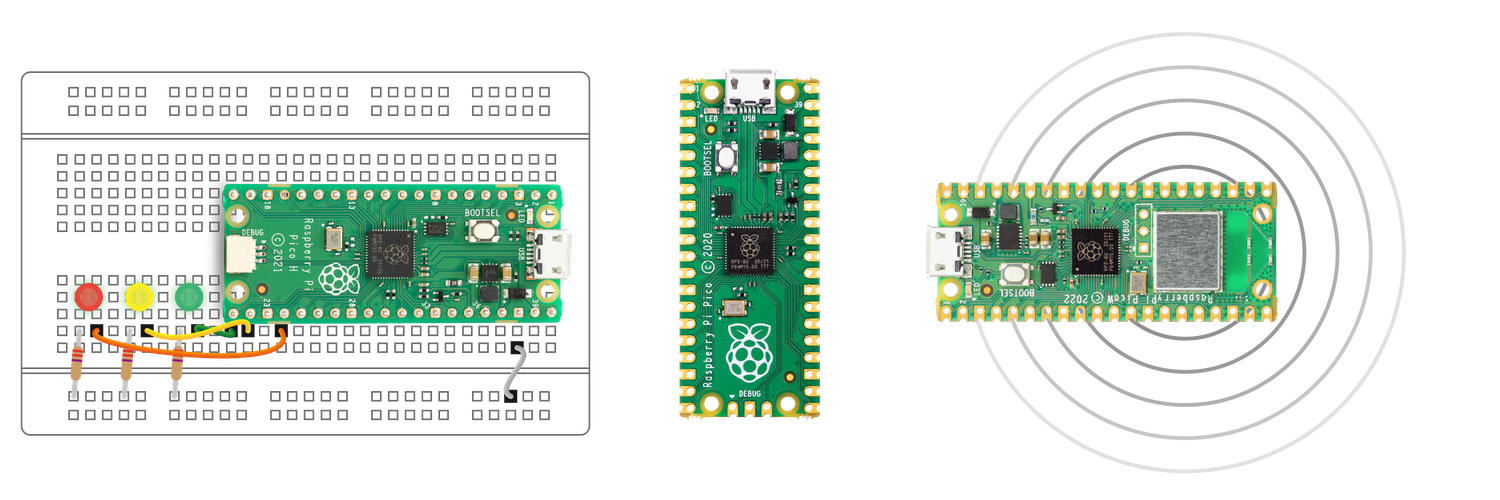
\includegraphics{rp2040.png} // zrobić fotkę mikrokontrolerowy
Mikrokontroler który wykorzystano to Raspberry Pico (RP2040)\cite{pico2024} w rozmiarze (z ang. form factor) 21 mm x 51 mm, z dwu-rdzeniowym procesorem Arm Cortex-M0+, z zegarem o maksymalnym taktowaniu 133 MHz. Ten "mini-komputer" posiada 264 kB SRAM-u i 2 MB pamięci QSPi, 26 wielofunkcyjnych pinów GPIO, włączając w to 3 wejścia analogowe.
Ponadto co jest szczególnie ważne w kwestii przyłączania zewnętrznych modułów mikrokontroler wyposażono w 2 UART, i co mniej ważne 2 SPI, 2 I2C i 16 kanałów PWM.
Do wgrywania programów udostępniono kontroler USB w wersji 1.1, z opcją hosta.
Obsługiwane napięcie wejściowe to od 1,8 V do 5,5 V DC.
Temperatura pracy to od -20 st. C do +85 st. C.
\section{Lora}
Jak podaje artykuł naukowy\cite{Augustin2016} LoRa to bezprzewodowy system telekomunikacyjny o dużym zasięgu, małej mocy i niskiej przepływności, promowany jako rozwiązanie infrastrukturalne dla Internetu rzeczy: urządzenia końcowe wykorzystują LoRa w pojedynczym przeskoku bezprzewodowym, aby komunikować się z bramą (bramkami), podłączonymi do Internetu, które działają jako przezroczyste mosty i przekazują wiadomości między tymi urządzeniami końcowymi a centralnym serwerem sieciowym. W artykule przedstawiono przegląd LoRa i dogłębną analizę jego funkcjonalnych komponentów.
W moim zastosowaniu nie będzie typowych bram, będą po prostu 2 urządzenia działające przy wykorzystaniu tego systemu.
LoRa jest ukierunkowana na zastosowania, w których urządzenia końcowe mają ograniczoną ilość energii (na przykład zasilane z baterii), w których urządzenia końcowe nie muszą przesyłać więcej niż kilka bajtów na raz i w których ruch danych może być inicjowany przez urządzenie końcowe lub przez podmiot zewnętrzny, który chce się z nim skomunikować. Charakter dalekiego zasięgu i niskiego poboru mocy LoRa sprawia, że jest to idealny kandydat do wykorzystania w tym projekcie.
LoRa zapewnia komunikację na duże odległości do 5 km w obszarach miejskich i do 15 km w obszarach wiejskich (w linii wzroku).
Protokół ten umożliwia tworzenie urządzeń, które na zasilaniu bateryjnym mogą działać nawet przez 10 lat.
\section{Bluetooth LE}
Jest to bezprzewodowa sieć osobista (PAN), zaprojektowana i stworzona przez Bluetooth Special Interest Group. Wykorzystuje się ją w opiece zdrowotnej, w branży fitness, w beaconach, bezpieczeństwie i urządzeniach domowej rozrywki. Jest niezależna od klasycznego Bluetooth i nie jest z nim kompatybilna, jednakże te dwie technologie mogą współdziałać w ramach pojedynczego urządzenia.
Sieć ta działa na częstotliwości 2,4 GHz, tak jak klasyczny Bluetooth.
Nominalny zasięg to poniżej 100 m, prędkość od 125 kbit/s do 2 Mbit/s, ilość urządzeń typu slave zależy od implementacji, do zabezpieczenia transmisji wykorzystywany jest 128-bitowy AES.
Sieć ta posiada aktywny frequency hopping, leniwe wiązanie, 24-bitowy klucz CRC i 32-bitowe sprawdzanie integralności wiadomości.
Ze stanu niepołączonego wybudza się w 6 ms, natomiast minimalny czas na wysłanie wiadomości to 3 ms.
Dostępna topologia to z ang. Scatternet.
Moc w zależności od przypadku użycia to 0,01-0,50 W.
Szczytowe natężenie prądu w czasie pracy to mniej niż 15 mA.
Główne zastosowania to telefony mobilne, gaming, inteligentny dom, urządzenia typu wearables, motoryzacja, komputery, bezpieczeństwo, urządzenia zbliżeniowe, ochrona zdrowia, sport, fitness i zastosowania przemysłowe.\cite{Wikipedia:ble:2024}
% !TeX encoding = UTF-8
% !TeX spellcheck = pl_PL
\chapter{Projekt urządzenia i oprogramowania}
\section{Schemat systemu}
%dołączyć schemat w formie grafiki, ew. poprawić opis
Mikrokontroler wkładany jest do gniazda w płytce z modułem Lora, wykorzystuje to 1 UART, do odrębnego UART-u podpinany jest z kolei moduł Bluetooth LE, którego wadą jest brak obsługi tzw. bondingu (modułu nie można powiązać przy użyciu PIN-u z pojedynczym urządzeniem, co jest pewną niedogodnością pod względem bezpieczeństwa).

% !TeX encoding = UTF-8
% !TeX spellcheck = pl_PL
\chapter{Badanie efektywności}
Badanie efektywności odbyło się dwojako. Przy użyciu symulacji numerycznej w programie Matlab, jak i poprzez eksperymenty w terenie.
\section{Symulacja numeryczna}
Wszystkie kody symulacji wykorzystane w pracy znajdują się w dodatku C.
Na poniższej grafice widać jak propaguje się sygnał na ścieżce wolnej, interesuje nas w szczególności część wykresu dla częstotliwości w okolicach 1 GHz, czyli takiej jaką wykorzystuje protokół Lora.
\begin{figure}[h!]
	\label{fig1}
	\includegraphics*{./grafika/num_sim1_straty_na_sciezce.png}
	\caption{Straty na ścieżce w wolnej przestrzeni}
\end{figure}


W rzeczywistości jednak sygnały nie poruszają się w próżni, więc straty na ścieżce wolnej opisują tylko część tłumienia sygnału.
Sygnały interferują z cząsteczkami w powietrzu i tracą energię na drodze propagacji. Straty różnią się w zaleźności od różnych czynników takich jak: ciśniecie, temperatura, opad atmosferyczny, rodzaj i gęstość opadu, zachmurzenie lub jego brak.

Poniżej znajduje się wykres przedstawiający tłumienie podczas opadu deszczu, na dystansie 5 km. Interesuje nas w szczególności część wykresu na jego początku, właśnie w takim zakresie częstotliwości, w jakim działa Lora.
\begin{figure}[h!]
	\label{fig2}
	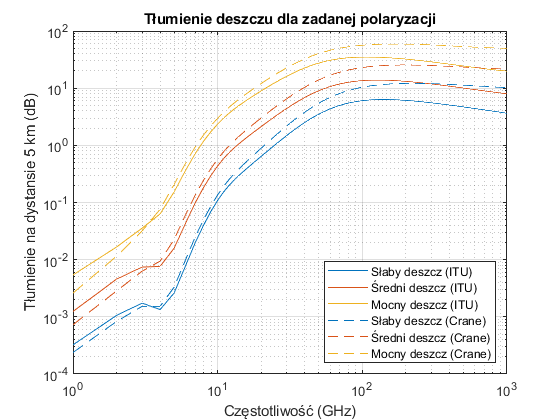
\includegraphics{./grafika/num_sim2_tlumienie_podczas_opadu_deszczu.png}
	\caption{Tłumienie deszczu dla zadanej polaryzacji na dystansie 5 km}
\end{figure}

Ponownie, poniżej wykresy, tym razem podczas opadu atmosferycznego w postaci śniegu, w 3 stopniach nasilenia, dla 2-óch odległości.
\begin{figure}[h!]
	\label{fig3}
	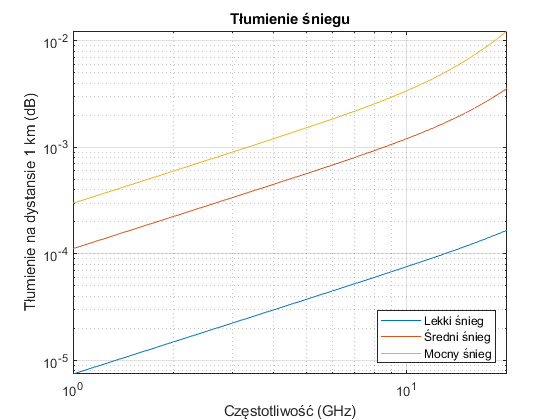
\includegraphics{./grafika/num_sim3_tlumienie_podczas_opadu_sniegu_1km.png}
	\caption{Tłumienie śniegu na dystansie 1 km}
\end{figure}

\begin{figure}[h!]
	\label{fig4}
	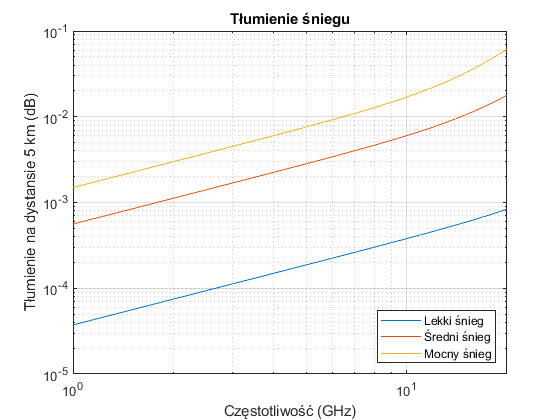
\includegraphics{./grafika/num_sim4_tlumienie_podczas_opadu_sniegu_5km.png}
	\caption{Tłumienie śniegu na dystansie 5 km}
\end{figure}


\section{Badanie terenowe}
% !TeX encoding = UTF-8
% !TeX spellcheck = pl_PL
\chapter{Podsumowanie}


%%%%%%%%%%%%%%%%%%%%%%%%%%%%%%%%%%%%%%%%%%%%%%%%%%%%%%%%%%%%%%%%%%%%%%%%%%%%%%%%%%%%%%%%%
%%%%%%%%%%%%%%%%%%%%%%%%%%%%%%%%%%%%%%%%%%%%%%%%%%%%%%%%%%%%%%%%%%%%%%%%%%%%%%%%%%%%%%%%%


%%% Polecenie \nocite{*} spowoduje umieszczenie w bibliografii wszystkich pozycji z bazy 
%%% nie zależnie od tego czy w tekście umieszczono do nuch odsyłacze. 
%\nocite{*}
\bibliographystyle{./bibliografia/plainurl}
\bibliography{./bibliografia/spis}

%%%%%%%%%%%%%%%%%%%%%%%%%%%%%%%%%%%%%%%%%%%%%%%%%%%%%%%%%%%%%%%%%%%%%%%%%%%%%%%%%%%%%%%%%

\cleardoublepage
\printnoidxglossary[nopostdot, sort=def, title=Wykaz symboli i skrótów]
%%%%%%%%%%%%%%%%%%%%%%%%%%%%%%%%%%%%%%%%%%%%%%%%%%%%%%%%%%%%%%%%%%%%%%%%%%%%%%%%%%%%%%%%%


%%%%%%%%%%%%%%%%%%%%%%%%%%%%%%%%%%%%%%%%%%%%%%%%%%%%%%%%%%%%%%%%%%%%%%%%%%%%%%%%%%%%%%%%%
\cleardoublepage
\listoffigures
%%%%%%%%%%%%%%%%%%%%%%%%%%%%%%%%%%%%%%%%%%%%%%%%%%%%%%%%%%%%%%%%%%%%%%%%%%%%%%%%%%%%%%%%%


%%%%%%%%%%%%%%%%%%%%%%%%%%%%%%%%%%%%%%%%%%%%%%%%%%%%%%%%%%%%%%%%%%%%%%%%%%%%%%%%%%%%%%%%%
\cleardoublepage
\listoftables
%%%%%%%%%%%%%%%%%%%%%%%%%%%%%%%%%%%%%%%%%%%%%%%%%%%%%%%%%%%%%%%%%%%%%%%%%%%%%%%%%%%%%%%%%
%\cftinserthook{lot}{BREAK}
\cleardoublepage

\appendix
%\addappheadtotoc
\appendixpage
\appendixtableofcontents

% tutaj dodatki o ile istnieją
\chapter{Tekst źródłowy programu na mikrokontroler}


\begin{lstlisting}[language=python,xleftmargin=0pt,  backgroundcolor={\color{white}}, caption={}, frame=""]
library ieee;
use ieee.std_logic_1164.all;
use ieee.std_logic_unsigned.all;
use ieee.std_logic_arith.all;

entity wave is
port (
  clk, reset : in std_logic;                           
  t_l, t_h   : in std_logic_vector(31 downto 0);  
  w          : out std_logic);
end wave;

architecture rtl of wave is
type FSM is (IDLE, PH, PL);
signal state, next_state: FSM;
signal timer : std_logic_vector(31 downto 0);
signal resetc: std_logic;

begin
RS_PROC:
process (clk, reset)
begin
  if (reset='0') then 
    state <= IDLE;
  elsif (rising_edge(clk)) then
    state <= next_state;
  end if;
end process;


NS_PROC:
process (state, t_l, t_h, timer)
begin
  case state is
  when  idle =>
  if (t_l = 0 or t_h = 0) then 
    next_state <= idle;
  else 
    next_state <= PH;
  end if;
  
  when PH =>  
  if (timer < t_h - 1) then  
    next_state <= PH;
  else
    next_state <= PL;
  end if;
    
  when PL =>
  if (timer < t_l - 1) then
    next_state <= PL;
  else
    next_state <= PH;    
   end if;    
end case;
end process;


DW_PROC:
process (state)
begin
  if    (state = PH) then   w <= '1';
  elsif (state = PL) then   w <= '0';
  end if;
end process;
end if;
end process;
end rtl;
\end{lstlisting}
\lstdefinelanguage{Kotlin}{
	comment=[l]{//},
	commentstyle={\color{gray}\ttfamily},
	emph={filter, first, firstOrNull, forEach, lazy, map, mapNotNull, println},
	emphstyle={\color{OrangeRed}},
	identifierstyle=\color{black},
	keywords={!in, !is, abstract, actual, annotation, as, as?, break, by, catch, class, companion, const, constructor, continue, crossinline, data, delegate, do, dynamic, else, enum, expect, external, false, field, file, final, finally, for, fun, get, if, import, in, infix, init, inline, inner, interface, internal, is, lateinit, noinline, null, object, open, operator, out, override, package, param, private, property, protected, public, receiveris, reified, return, return@, sealed, set, setparam, super, suspend, tailrec, this, throw, true, try, typealias, typeof, val, var, vararg, when, where, while},
	keywordstyle={\color{NavyBlue}\bfseries},
	morecomment=[s]{/*}{*/},
	morestring=[b]",
	morestring=[s]{"""*}{*"""},
	ndkeywords={@Deprecated, @JvmField, @JvmName, @JvmOverloads, @JvmStatic, @JvmSynthetic, Array, Byte, Double, Float, Int, Integer, Iterable, Long, Runnable, Short, String, Any, Unit, Nothing},
	ndkeywordstyle={\color{BurntOrange}\bfseries},
	sensitive=true,
	stringstyle={\color{ForestGreen}\ttfamily},
}
\chapter{Kod źródłowy aplikacji na telefon z systemem operacyjnym Android}

\begin{lstlisting}[language=Kotlin, xleftmargin=0pt, backgroundcolor={\color{white}}, caption={}, frame=""]
library ieee;
use ieee.std_logic_1164.all;
use ieee.std_logic_unsigned.all;
use ieee.std_logic_arith.all;

entity shift_reg is
generic(N: integer range 0 to 32 := 8);
port (
clk, reset, load  : in  std_logic;
pos, reg_in       : in  std_logic_vector(N-1 downto 0);
reg_out           : out std_logic_vector(N-1 downto 0));
end shift_reg;

architecture rtl of shift_reg is
signal rejestr: std_logic_vector(N-1 downto 0);

begin
process (clk, reset, load, reg_in)
begin
  if (reset = '0') then 
    rejestr <= (others => '0');
   elsif (load = '0') then
     rejestr <= reg_in;
   elsif (rising_edge(clk)) then
     rejestr (N-1 downto conv_integer(pos)) <= rejestr(N-1-conv_integer(pos) downto 0);
     rejestr (conv_integer(pos) downto 0)   <= (others => '0');
  end if;
end process;

reg_out <= rejestr;
end rtl;
\end{lstlisting}



\end{document}

